\section{基于邻域的回归}
\label{sec:regression-instance}

全局线性模型假设同一条直线或平面适用于整个输入空间；真实关系可能在不同区域弯曲、转折，统一参数反而处处拟合不好。基于邻域的回归放弃全局参数，只为查询点$\bm{x}_\star$找出附近的训练记录，用它们的局部信息作预测。近邻表示与检索的基础见第\ref{sec:classic-overview-neighborhood}节。

\subsection{k近邻回归}
\label{sec:regression-knn}

\subsubsection{模型结构}
\label{sec:regression-knn-structure}

\term{$k$近邻回归}（$k$-nearest neighbor regression）保存全部训练实例，按距离找出与$\bm{x}_\star$最近的$k$条记录，取其响应平均：
\begin{equation}
  \widehat f(\bm{x}_\star)
  =\frac{1}{k}\sum_{i\in N_k(\bm{x}_\star)}y_i,
  \label{eq:regression-knn}
\end{equation}
其中$N_k$为恰含$k$条记录的邻居集合，输出为数值响应平均；距离可取欧氏距离或\term{马氏距离}（Mahalanobis distance，按各特征方差归一化后的距离，量纲大的特征不会天然占优）。距离计算前先按训练折标准化各特征尺度，避免量纲主导，并列与零距离另有约定。$k=1$逐点跟随最近记录，$k=n$退化为整体均值，两端分别对应高方差与高偏差。

\subsubsection{参数学习}
\label{sec:regression-knn-learning}

\paragraph{训练记录与邻域配置}

kNN没有显式训练，训练集本身就是模型：明确训练记录保存和预处理，在训练折内选择邻居数$k$与距离配置，验证点不进入自己的邻居库。没有固定维数系数拟合，仍需学习配置并保存可用的参考记录。

\paragraph{查询与检索实现}

预测时计算$\bm{x}_\star$到全部记录的距离并排序，处理平局并聚合响应；朴素扫描的代价为$O(n)$，有效邻居不足时按约定返回。在相同预测规则下比较精确树索引与近似检索，交代维数、数据几何和查询预算的影响；近似检索可能改变邻居及输出，速度收益与预测误差分别核验，不另造一种回归模型。标准化参数只来自训练折。

\subsubsection{理论分析}
\label{sec:regression-knn-theory}

\paragraph{有限邻域的误差分解}

在输入决定邻居、条件独立零均值噪声与方差有界的设定下，把误差分为邻域函数变化与噪声平均：$k$小则局部追随训练波动，估计方差大、偏差小；$k$大则平均平滑，方差小但可能把远处无关记录也平均进来，偏差增大，由此得到给定输入的Lipschitz偏差—方差界。高维空间中所有点彼此距离相近，邻居不再"近"，这是维数灾难下kNN失效的原因——特征很多时任意两点距离都差不多，"近邻"不再真的近。重复抽样下的偏差—方差分解与第\ref{sec:regression-regularization}节一致，不给无条件排序。

\paragraph{样本增加时的一致性}

有限维欧氏输入、独立同分布、有限响应二阶矩及适当并列规则下，$k$增长而$k/n$下降时估计一致；区分点处几何条件、总体积分误差与有限样本结论。

\paragraph{支持距离加权}
\label{sec:regression-knn-weighted}

等权平均忽略邻居远近，引入非负距离权重并归一化，写加权响应均值及零距离处理：越近的邻居权重越大，$w_i=\exp(-d_i^2/(2h^2))$，再加权平均，避免等权抹平近处信息。固定输入与权重后，从独立噪声求条件方差，说明权重过度集中怎样改变方差。在相同邻居库和查询点比较等权、较缓衰减与较强衰减，分别讨论局部变化、标签噪声和训练内配置选择；不能仅凭距离更近保证响应更可靠，检索索引改变的是计算。

\subsection{局部加权回归（LOESS）}
\label{sec:regression-loess}

kNN只对邻居响应作常数平均，在查询位于一段倾斜趋势上时，平均会落在段内中点而非查询处。\term{局部加权回归}（LOESS，局部回归）在邻域内拟合一条局部直线，让查询处的切线反映局部斜率。Cleveland在1979年给出稳健局部回归的系统形式\scite{cleveland1979lowess}。

\subsubsection{模型结构}
\label{sec:regression-loess-structure}

对查询$\bm{x}_0$，在其邻域内最小化核加权局部多项式目标
\begin{equation}
  \sum_{i=1}^n K_h(\bm{x}_i-\bm{x}_0)
    \left[y_i-b-\bm{w}^{\top}(\bm{x}_i-\bm{x}_0)\right]^2,
  \label{eq:regression-local-polynomial}
\end{equation}
$K_h$为带宽$h$的核权重，距离越近权重越大；常数、一次、二次分别改变局部表达能力，一次局部线性在$\bm{x}_0$处给出预测$b$。距离权重核与特征内积核含义不同，带宽决定局部有效样本范围，新查询会改变局部问题。

\subsubsection{参数学习}
\label{sec:regression-loess-learning}

固定查询点构造加权局部设计，推导正规方程及一维局部线性预测权重，说明正权输入数和局部秩条件；每个查询点独立解一次加权最小二乘，可用加权QR等解系数，有效点不足时扩邻域或降阶回退。带宽（邻域跨度）、阶数和预处理由训练内验证确定，交代每次查询的搜索与重拟合代价，核函数形式固定。

\subsubsection{理论分析}
\label{sec:regression-loess-theory}

由式\eqref{eq:regression-local-polynomial}求和可得$\sum_i l_i=1$、$\sum_i l_i(x_i-x_0)=0$。所以对于一次函数$m(x)=a+bx$，即使邻居都在查询的一侧，仍有$\sum_i l_i m(x_i)=m(x_0)$；局部斜率消去了平均输入不等于查询输入带来的一阶偏差。对光滑曲线，Taylor展开的常数项与一次项同样被再现，剩下的是曲率与更高阶变化\scite{fan1996local}。给固定输入权重下的条件方差并说明预测权重可能为负、退化局部设计会放大噪声，偏差下降不保证总误差下降。

\paragraph{局部常数特例：Nadaraya–Watson平滑}
\label{sec:regression-nadaraya-watson}

邻域中若只有一个有效输入，局部斜率无法确定；即使样本更多，估计斜率也可能带来不需要的噪声放大。只保留局部常数就能减少待估参数，同时保留按距离区别观测的方式。在式\eqref{eq:regression-local-polynomial}中只拟合截距，对截距求导便得到\term{Nadaraya--Watson核平滑}（Nadaraya--Watson kernel smoothing）
\begin{equation}
  \widehat f(\bm{x}_0)
  =\frac{\sum_i K_h(\bm{x}_i-\bm{x}_0)y_i}
         {\sum_i K_h(\bm{x}_i-\bm{x}_0)},
  \label{eq:regression-nw}
\end{equation}
分子核加权响应和，分母核权重和归一化。Nadaraya与Watson在1964年分别提出这一估计\scite{nadaraya1964,watson1964}。对照局部线性解释单侧偏差与方差取舍，区分距离权重核与内积核；边界处邻居只来自一侧，核权重和偏小，常数估计产生边界偏差，局部线性的一阶再现能缓解这一问题。图\ref{fig:regression-neighborhood}展示邻居搜索与局部平均的关系。

\begin{figure}[htbp]
  \centering
  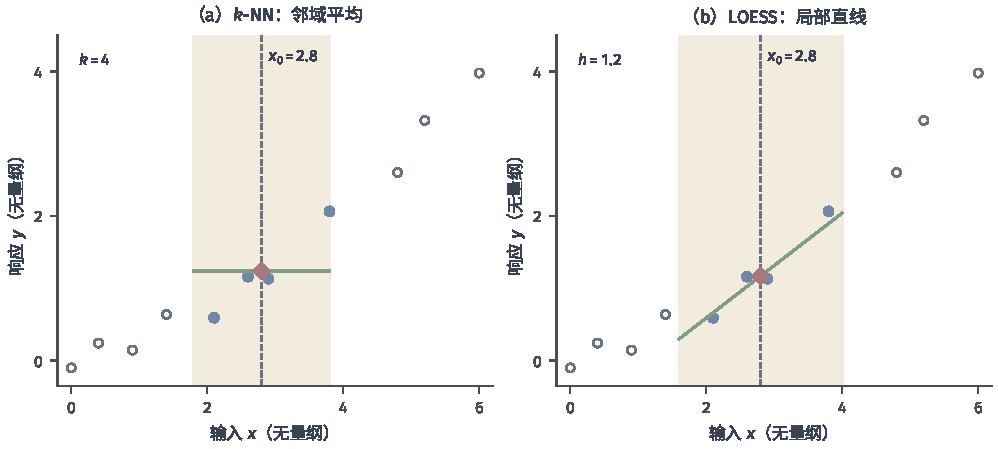
\includegraphics[width=105.412mm]{figures/04-classic-models/00-shared/matplotlib/regression-neighborhood/figure.pdf}
  \caption{邻域回归的查询几何。星号为查询点，圆圈为训练样本，浅色圆标出邻域；预测由邻域内记录按距离加权平均或局部拟合得到。远离查询的记录不参与。}
  \label{fig:regression-neighborhood}
\end{figure}

\paragraph{支持异常响应：稳健LOESS}
\label{sec:regression-loess-robustness}

局部拟合同样会被邻域内的异常响应带偏：距离近不等于响应可靠。稳健LOESS在局部线性拟合之后，按残差大小重新赋权：给残差双权重（bisquare）和尺度来源，大残差记录用双权重函数压到接近零，再重新拟合，按距离拟合、计算残差、增加降权、重新拟合完整说明循环与停止，迭代若干轮。这样异常点在后续轮次几乎不参与局部直线，而不必在全局删除样本；响应依赖权重后不能沿用固定线性算子结论。稳健权重与带宽、局部阶数一起由训练内验证控制。
